\chapter{Metodologia}
\label{cap:03}

Este capítulo apresenta o método da pesquisa e o processo de desenvolvimento da extensão GUY. Primeiro, delimita-se o objeto de análise e a forma de avaliação; em seguida, descrevem-se as atividades de construção da ferramenta, sem confundir o procedimento de pesquisa com as decisões de implementação.

\section{Método da Pesquisa}
\label{sec:metodo_pesquisa}

Trata-se de uma pesquisa aplicada, de caráter exploratório e descritivo, conduzida por meio da construção e da avaliação técnica de uma ferramenta de análise estática. O objeto de análise é o código Python apresentado ao GUY no VS Code, nos escopos de arquivo, seleção ou função atual. A avaliação não envolve a execução dos programas: verifica a correspondência entre as estruturas de controle reconhecidas, o GFC construído e o valor da Complexidade Ciclomática.

Para a validação, foram utilizados os três arquivos de exemplo disponíveis em \texttt{src/examples/}, que representam diferentes combinações de estruturas de controle em Python. Para cada exemplo, os nós, as arestas, as decisões, os componentes e os caminhos independentes foram confrontados com uma reconstrução manual baseada na convenção de modelagem do GFC e com a fórmula de $V(G)$. Portanto, os resultados sustentam conclusões apenas para esses exemplos e para o escopo implementado.

\section{Ambiente de Avaliação e Reprodutibilidade}
\label{sec:ambiente_avaliacao}

Os registros experimentais foram produzidos em 24 de julho de 2026 com a versão \texttt{v0.1.1c} do GUY, correspondente ao commit \texttt{96afe6a4a9896624025d1b082048f6f2141c40d6} do repositório \texttt{gm64x/guy-vscode}. Esse estado era a versão funcional mais recente disponível no GitHub antes da inclusão das capturas no documento. O ambiente utilizou Visual Studio Code 1.127 e Node.js 24.18.0 LTS. Os testes foram realizados no Windows 11, versão 24H2 (build 26100), e no Ubuntu 26.04 LTS (Resolute Raccoon).

O arquivo de dependências travadas dessa versão registra React 19.2.7, \texttt{@xyflow/react} 12.11.0, \texttt{@dagrejs/dagre} 3.0.0, Tree-sitter 0.22.4, \texttt{tree-sitter-python} 0.23.6 e \texttt{web-tree-sitter} 0.26.9. A identificação conjunta da tag, do commit, do ambiente e das dependências relaciona os resultados apresentados à versão efetivamente avaliada, ainda que versões posteriores da extensão possuam funcionalidades adicionais.

\section{Panorama Geral da Pesquisa}
Como ilustrado na Figura \ref{fig:fluxo_GUY}, o GUY permite que estudantes e profissionais gerem Grafos de Fluxo de Controle (GFCs) a partir do arquivo aberto no \textit{Visual Studio Code} (VS Code). Com isso, a extensão apoia o estudo da lógica interna do código e o planejamento de testes estruturais durante o desenvolvimento.

\begin{figure}[htbp]
\centering
\caption{Fluxo de funcionamento da ferramenta proposta.}
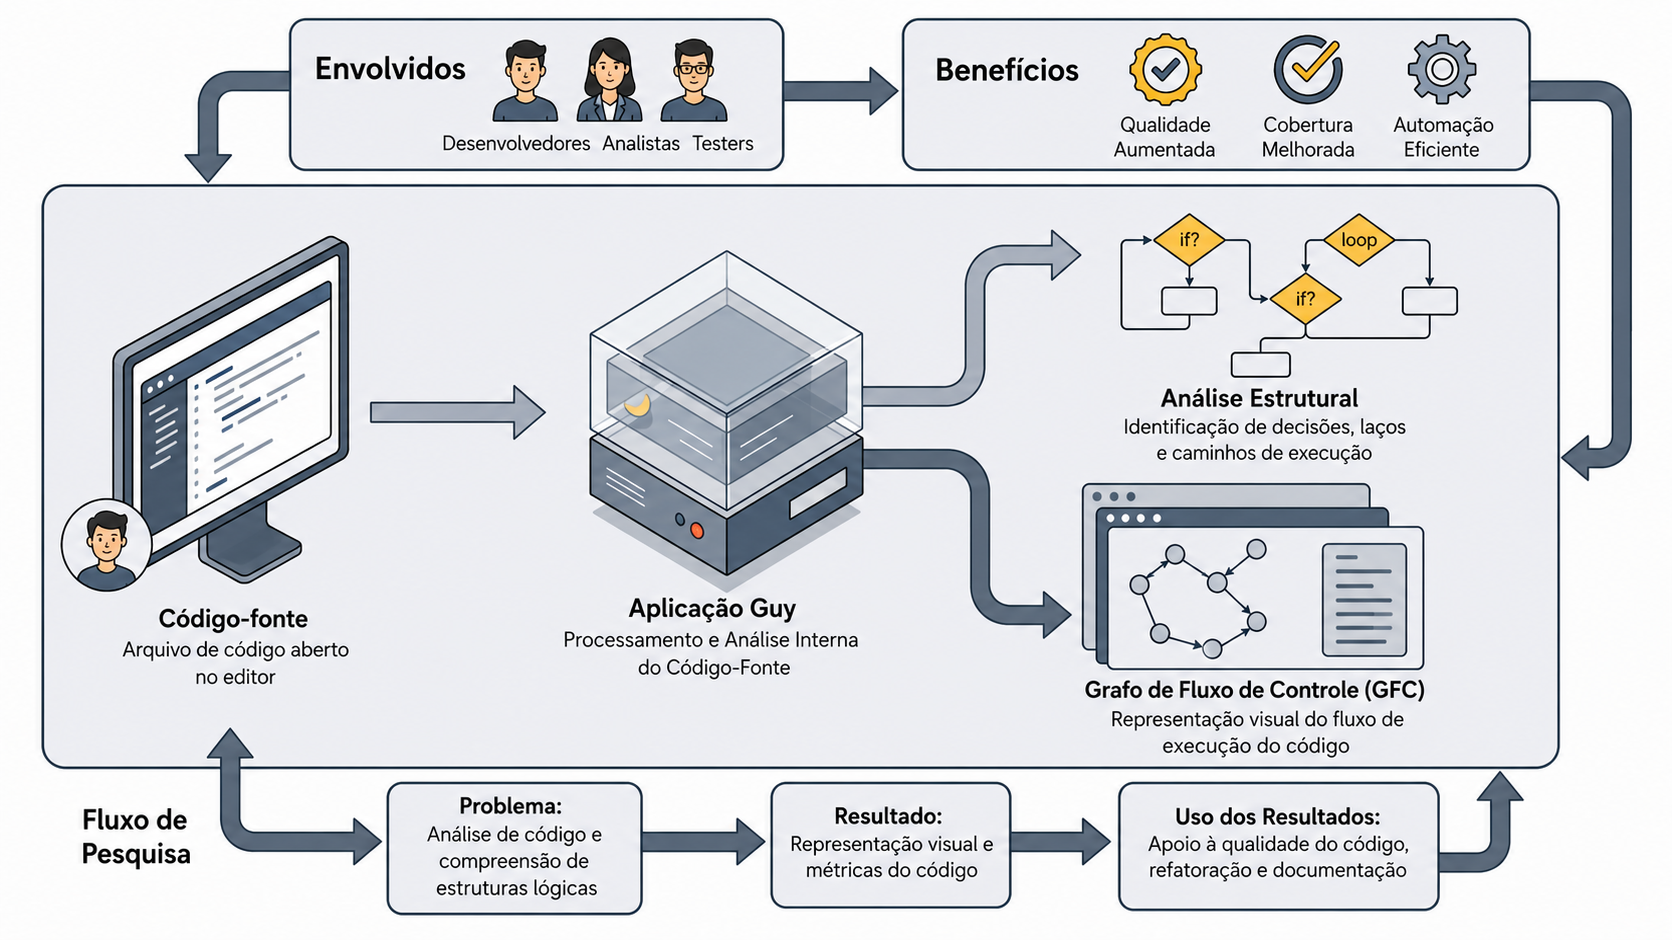
\includegraphics[width=0.75\linewidth]{imagens/fluxos/fluxo_guy.png}

\fonte{Elaborada pelo autor (2025).}
\label{fig:fluxo_GUY}

\end{figure}

A ferramenta é acionada a partir do arquivo de código-fonte aberto no editor. Em seguida, o núcleo de processamento do GUY executa a análise estática local, mapeia as estruturas lógicas do algoritmo e constrói a representação visual do Grafo de Fluxo de Controle. Essa representação permite identificar os nós de decisão e os caminhos de execução possíveis no trecho analisado.

Com o GFC estruturado, o usuário passa a visualizar os caminhos independentes do algoritmo. Essa visualização integrada oferece a estudantes, desenvolvedores e analistas de qualidade (\textit{testers}) os fluxos que podem orientar o estudo e a elaboração de casos de teste estruturais.

As decisões de construção são detalhadas no Capítulo \ref{cap:04}, enquanto o protocolo de validação e os resultados experimentais são apresentados no Capítulo \ref{cap:05}.
